\chapter{经典模型概述}
\label{chap:classic-models-overview}

给定一批房屋成交记录，我们可以根据面积、楼龄和位置预测价格，也可以判断房屋属于哪个预设的价格档位。撤去价格和类别后，同一批属性还可以用于寻找相似房屋，或压缩成少数便于观察的坐标。预测数值、判断类别、发现群组和压缩表示，是四种不同的任务；它们却常用到相同的计算，例如特征加权、邻居搜索和条件划分。本章考察这些计算怎样构成模型，以及任务改变后，输出含义与学习准则为什么也要改变。

\section{经典模型的历史}
\label{sec:classic-overview-history}

从观测中建立模型，需要同时决定用什么表示规律、怎样估计这种表示中的未知量。早期统计方法常把规律写成少量系数，后来的方法则更多地利用局部样本、输入分区或多个分布成分。这些变化扩展了可选择的表示，并没有使早期方法失效：当数据主要包含全局趋势时，少量系数仍便于估计；当不同区域遵循不同关系时，局部或分区表示才有必要。

\subsection{从统计估计到局部与分区模型}
\label{sec:classic-history-statistical}

最小二乘、回归与判别分析建立了“先规定函数形式，再用数据估计系数”的主干。线性关系便于计算和解释，也能通过概率假设描述误差。目标包含局部变化时，一个全局系数向量可能受限；近邻方法直接利用查询点附近的记录，树方法则按输入条件把不同局部预测组织起来。前者把训练样本保留为预测依据，后者把样本归纳成可重复执行的规则，二者改变了模型存储和使用数据的方式\scite{hastie2009}。

没有价格或类别标签时，模型缺少可直接比较的预测答案，需要另外规定要保留的数据结构。主成分分析用少量投影方向保留输入中的主要变化；聚类可以按到代表点的距离、邻域密度、群组的包含关系或分布成分来组织样本。它们得到的分组或坐标可能不同，因为所要求保留的关系不同。评价无监督模型也要回到这一要求，不能把一种分组当作所有任务的唯一答案\scite{bishop2006}。

\subsection{从非线性表示到模型组合}
\label{sec:classic-history-kernel-ensemble}

非线性并不一定要求放弃线性求解。核方法把内积替换为能够隐式表达特征交互的函数，在新的特征空间中继续使用线性预测或几何准则。1995年的支持向量网络把这一思路与最大间隔分类联系起来，之后同样的核几何也用于回归、聚类与降维\scite{cortes1995}。

一棵树可能因训练样本的少量改变而得到不同划分，单个简单模型也可能留下尚未拟合的规律。1996年的Bagging通过重采样训练多个成员，再聚合预测，以减弱不稳定成员的波动。2001年的随机森林在此基础上随机选择节点的候选特征，减少各棵树采用相同划分的机会。梯度提升则逐轮添加成员，让新增预测沿着所选损失的下降方向修正整体模型。现代树集成还改进正则化、稀疏统计和训练实现；这些改动节省多少计算、是否降低新样本误差，需要分别检验\scite{breiman1996bagging,breiman2001randomforests,friedman2001gradientboost}。

图\ref{fig:classic-models-history}把这些路线放在一条时间路径上。时间表示代表工作出现的先后，分组说明它改变了表示、学习或组合中的哪个环节；它不是方法优劣或淘汰顺序。
\begin{figure*}[p]
  \centering
  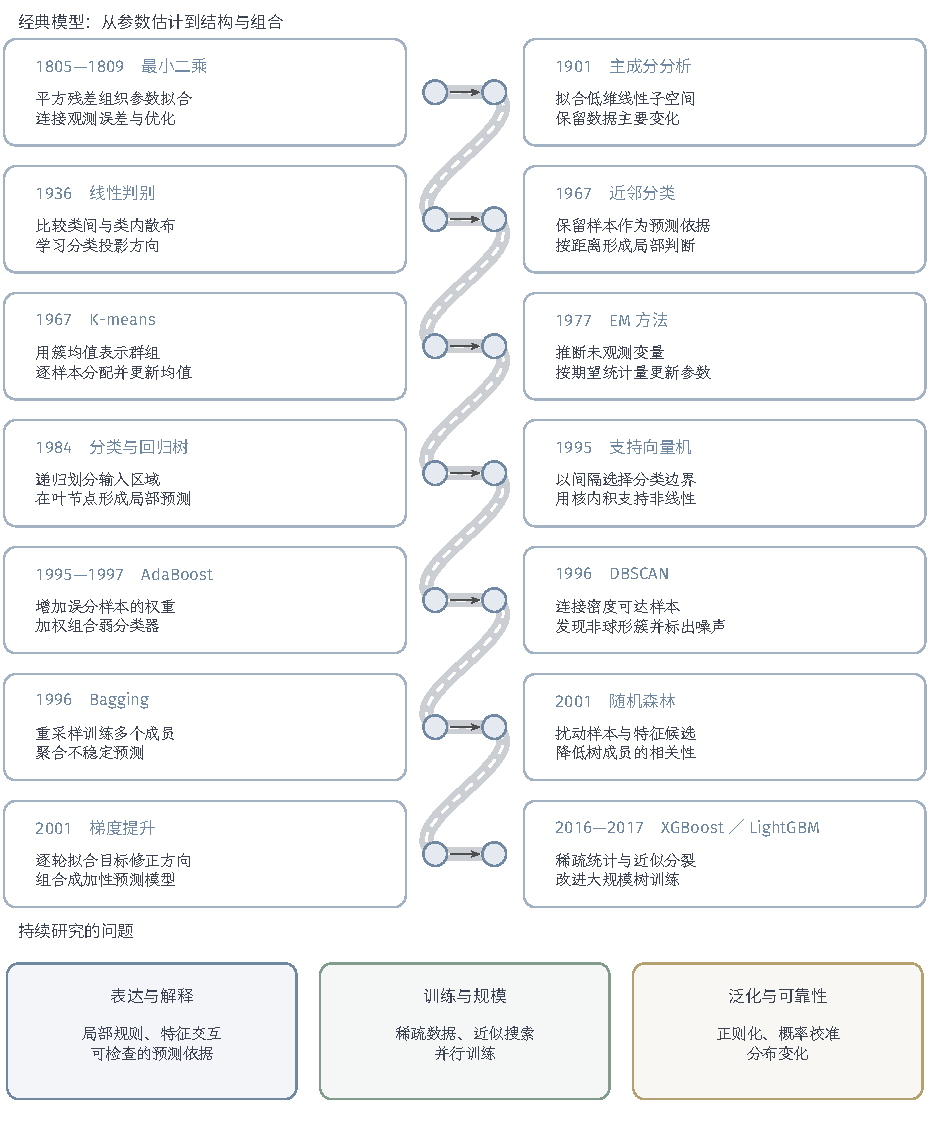
\includegraphics[width=157.406mm,height=.82\textheight,keepaspectratio]{figures/03-models/01-classic-models/tikz/classic-models-history/figure.pdf}
  \caption{经典模型的代表性发展节点。沿时间路径可观察参数估计怎样扩展到结构发现、局部预测、非线性表示和模型组合。节点间距不表示实际时间长度，年份对应代表工作；这些方法持续交叉使用，并非依次替代。底部列出仍需分别评价的表达、训练与预测问题。}
  \label{fig:classic-models-history}
\end{figure*}
\FloatBarrier

\section{经典模型的类型}
\label{sec:classic-overview-modeling}

以房屋数据为例，预测器可以假定面积等属性共同形成一个全局趋势，也可以主要参考相似房屋，或针对不同条件学习不同的局部规则。概率模型进一步说明相同输入下结果可能怎样变化，集成方法则组合多个成员的判断。这些思路允许交叉：一个模型可以同时使用线性关系和概率分布，也可以把树作为集成成员。下面沿着它们各自回答的问题，说明共享结构怎样随任务改变。

\subsection{基于线性关系的建模}
\label{sec:classic-overview-linear}

预测房价时，一个直接的起点是给面积、楼龄等特征分别赋予权重，再相加得到预测。设输入为$\bm{x}\in\mathbb{R}^{d}$，权重为$\bm{w}\in\mathbb{R}^{d}$，偏置为$b\in\mathbb{R}$，这个计算写成
\begin{equation}
  g(\bm{x})=\bm{w}^{\top}\bm{x}+b.
  \label{eq:classic-overview-linear-score}
\end{equation}
在线性回归中，$g(\bm{x})$可以直接作为价格预测；在二分类中，它可以作为类别得分，再按阈值给出类别。加权求和的结构相同，但回归系数需要贴合数值响应，分类权重需要帮助区分类别。得分也可以经适当转换得到类别概率，这就与后面的概率建模相接。

当目的从预测变成降维时，加权求和仍然有用，只是输出改为少数新的坐标。主成分分析（principal component analysis, PCA）选择若干投影方向，让保留的坐标描述数据的主要变化；这里学习方向的依据是输入自身的变化，而不是房价或类别标签。第\ref{sec:dim-pca}节会说明这一目标与重构误差的关系。同样的线性运算并不意味着相同的学习问题。

如果大户型和小户型的面积增量对应不同的价格变化，或面积的作用取决于楼龄，原始特征的加权和就可能过于受限。可以先加入面积平方、面积与楼龄的乘积等新特征，再学习它们的权重。这种\term{特征映射}（feature mapping）把原来的输入改写成另一组可供计算的特征，使简单的线性组合也能表达原始输入中的非线性关系。线性因而要相对于所用的特征来判断；第\ref{sec:regression-basis}节从基函数展开说明这种扩展。

平方项和交互项越多，显式保存的特征向量就越长。有些训练和预测过程只需要两份特征向量的内积，因而无需分别生成它们：只要有一个函数直接返回同样的内积，就能完成原来的计算。这类\term{核方法}（kernel method）通过内积函数指定特征空间，省去显式展开的成本。下面从一个圆形分类边界说明这种转换，再检查什么样的函数能够充当内积。

图\ref{fig:classification-kernel-map}用一个二维分类例子展示特征映射$\bm{\phi}(\bm{x})=(x_1,x_1^2+x_2^2)^{\top}$。输入空间中的圆$x_1^2+x_2^2=1$，在新坐标中变成直线$\phi_2=1$；同一得分$g(\bm{x})=1-x_1^2-x_2^2$于是可以写成$g(\bm{x})=(0,-1)\bm{\phi}(\bm{x})+1$。改变的是输入的表示，原来位于圆内与圆外的样本不需要改变类别。这幅图给定了一条可行边界，用于解释几何对应，不把它当作训练后的最大间隔解。

\begin{figure}[htbp]
  \centering
  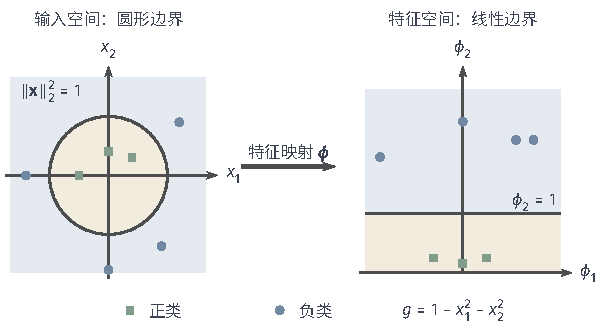
\includegraphics[width=103.166mm]{figures/04-classic-models/00-shared/tikz/classification-kernel-map/figure.pdf}
  \caption{非线性边界在特征映射前后的对应，两个面板的坐标均无量纲。正类方点为$(-0.5,0)$、$(0,0.4)$、$(0.4,0.3)$，负类圆点为$(-1.4,0)$、$(0,-1.6)$、$(1.2,0.9)$、$(0.9,-1.2)$。右图逐点使用$\phi_1=x_1$、$\phi_2=x_1^2+x_2^2$；水平线$\phi_2=1$对应左图半径为1的圆。数据与边界均为教学构造。}
  \label{fig:classification-kernel-map}
\end{figure}

\subsubsection{特征映射与核技巧}
\label{sec:classic-overview-kernel-trick}
\label{sec:classification-svm-kernel-trick}

圆形边界的例子显式增加了一个平方特征；当特征更多时，逐一构造坐标可能成为计算负担。设特征映射$\bm\phi:\mathbb R^d\to\mathcal H$把输入送到带内积的特征空间，在那里使用线性预测器$f(\bm x)=\langle\bm w,\bm\phi(\bm x)\rangle+b$。若学习过程得到的权重可以写为$\bm w=\sum_{i=1}^n a_i\bm\phi(\bm x_i)$，代入预测式后，每个训练样本只通过一个特征内积参与计算：
\begin{equation}
  f(\bm x)=\sum_{i=1}^{n}a_iK(\bm x_i,\bm x)+b,
  \qquad K(\bm x,\bm z)=\langle\bm\phi(\bm x),\bm\phi(\bm z)\rangle_{\mathcal H}.
  \label{eq:classic-overview-kernel}
\end{equation}
这里$a_i$由具体学习目标确定，核$K$直接返回两份特征的内积。用核值替换特征内积的做法称为\term{核技巧}（kernel trick）。它不改变分类、回归或降维的目标，而是让这些目标在新的几何中计算；$K$对原输入可以非线性，预测也就能够具有非线性边界。只有计算可以写成这些内积时，才可直接作这种替换。

例如$K(\bm x,\bm z)=(\bm x^\top\bm z)^2$隐含平方项与交互项。训练时可以计算$n\times n$的核矩阵，再按具体目标求系数；预测时计算新输入与训练输入的核值，并按式\eqref{eq:classic-overview-kernel}加权。这省去了二次特征的显式展开，却将计算与存储转到了样本之间的关系上。无限维映射也可以用这种形式计算，其代价同样取决于需要访问多少训练样本（特征空间的背景参考\BookChapterRef{chap:functional-analysis-and-approximation}{第一卷“数学准备”的“函数空间”章}）。

\subsubsection{用正定核构造非线性特征空间}
\label{sec:classic-overview-kernel-validity}
\label{sec:classification-svm-mercer}

用函数$K$替代内积以后，还需要确认这个替代保持了内积的几何性质。特征向量线性组合的范数平方应当非负，因此对任意有限输入与实系数都必须有$\sum_{i,j}a_i a_jK(\bm x_i,\bm x_j)\geq0$；内积的对称性还要求$K$对称。这些条件使任意有限Gram矩阵半正定，也保证能在某个Hilbert空间中构造出相应特征内积。由此可以直接设计$K$，而不必先列出全部特征坐标（构造依据参考\BookTheoremRef{thm:functional-moore-aronszajn-construction}{第一卷“数学准备”的“正定核的RKHS构造”定理}）。

本书的“正定核”允许Gram矩阵奇异；需要排除互异输入下的退化时，才要求严格正定。半正定回答的是能否构造特征内积。核矩阵的可逆性、目标的求解难度和表示对任务的适合程度，则分别取决于数据、学习目标与核的选择。正则化和选解规则处理求解中的退化，核尺度等超参数通过独立验证选择。

非负加权和、核的乘积及逐点有限极限可以构造新核，分别对应特征直和、张量积及有限二次型极限。这些规则可以把多个信息来源组合成一个合法内积。某份训练集的矩阵通过检查，只认证这一组点；预测还会遇到新输入，因此核应在整个预期定义域上具有构造依据。在非空紧度量输入域上，若核连续，并使用有限、全支撑的Borel测度，可用Mercer展开得到显式谱坐标（参考\BookTheoremRef{thm:functional-mercer}{第一卷“数学准备”的“连续正定核的Mercer展开”定理}）。核技巧本身不要求先求出谱展开。

\subsubsection{常用核与表示选择}
\label{sec:classic-overview-common-kernels}
\label{sec:classification-svm-common-kernels}

回到$\bm{x},\bm{z}\in\mathbb{R}^d$。常用核之间的区别主要在于怎样度量接近程度、允许哪些特征交互，以及这些选择带来怎样的函数范数。表\ref{tab:classification-svm-kernels}列出五种常见形式，核尺度统一记为$\beta$，多项式次数记为$p$，避免与输入维数$d$混用。

\begin{table}[htbp]
  \centering
  \small
  \begin{tabularx}{\linewidth}{@{}>{\RaggedRight\arraybackslash}p{18mm}>{\RaggedRight\arraybackslash}X>{\RaggedRight\arraybackslash}p{27mm}@{}}
    \toprule
    名称 & $K(\bm{x},\bm{z})$ & 参数与正定性\\
    \midrule
    线性核 & $\bm{x}^{\top}\bm{z}$ & 半正定\\
    多项式核 & $(\beta\bm{x}^{\top}\bm{z}+r)^p$ & $\beta,r\ge0$，正整数$p$\\
    高斯RBF核 & $\exp(-\beta\lVert\bm{x}-\bm{z}\rVert_2^2)$ & $\beta>0$，半正定\\
    Laplacian核 & $\exp(-\beta\lVert\bm{x}-\bm{z}\rVert_1)$ & $\beta>0$，半正定\\
    Sigmoid形式 & $\tanh(\beta\bm{x}^{\top}\bm{z}+r)$ & 一般不保证半正定\\
    \bottomrule
  \end{tabularx}
  \caption{常用核函数与合法性条件。这里的“半正定”要求任意有限输入的Gram矩阵半正定；Sigmoid一行列出的是常见相似性形式，使用前仍需针对定义域与参数核验。}
  \label{tab:classification-svm-kernels}
\end{table}

\term{线性核}（linear kernel）对应$\bm{\phi}(\bm{x})=\bm{x}$，保留原始特征内积。对于线性预测，训练样本的核展开可以先聚合为一个权重向量，使用时只需与新输入作内积。是否加入非线性交互，取决于原特征中的线性组合能否描述目标规律；验证数据可以比较这两种表示在相同预测任务上的误差。输入维数只是表示的规模，本身没有回答哪种关系更适合任务。

\term{多项式核}（polynomial kernel）把有限阶交互隐式加入模型。以$d=2$、$\beta=1$、$r=0$、$p=2$为例，
\[
  \begin{aligned}
    (\bm{x}^{\top}\bm{z})^2
      &=x_1^2z_1^2+2x_1x_2z_1z_2+x_2^2z_2^2,\\
    \bm{\phi}(\bm{x})
      &=(x_1^2,\sqrt2\,x_1x_2,x_2^2)^{\top}.
  \end{aligned}
\]
交叉项前的$\sqrt2$使特征内积准确等于核值。一般地，令多重指标$\bm{a}=(a_1,\ldots,a_d)$满足$|\bm{a}|=\sum_j a_j=p$，并记$\bm{x}^{\bm{a}}=\prod_j x_j^{a_j}$、$\bm{a}!=\prod_j a_j!$。多项式展开为
\[
  (\bm{x}^{\top}\bm{z})^p
  =\sum_{|\bm{a}|=p}\frac{p!}{\bm{a}!}
     \bm{x}^{\bm{a}}\bm{z}^{\bm{a}}.
\]
所以齐次$p$次核可以使用$\binom{d+p-1}{p}$个单项式坐标；当$\beta>0,r>0$时，非齐次核包括$0$至$p$次项，一种完整单项式表示的维数是$\binom{d+p}{p}$。这些是特征数量，不是样本数量；计算一个核值通常只需一次$d$维内积和幂运算，节省的是显式特征展开成本，完整优化仍要另计。

\term{高斯径向基核}（Gaussian radial basis function kernel，Gaussian RBF kernel）根据欧氏距离赋予局部相似性。其无限维特征可以由指数级数直接看出：
\begin{equation}
  \begin{aligned}
    K(\bm{x},\bm{z})
      ={}&e^{-\beta\lVert\bm{x}\rVert_2^2}
          e^{-\beta\lVert\bm{z}\rVert_2^2}\\
       &\cdot\sum_{p=0}^{\infty}
          \frac{(2\beta)^p}{p!}
          (\bm{x}^{\top}\bm{z})^p.
  \end{aligned}
  \label{eq:classification-svm-rbf-expansion}
\end{equation}
每一阶多项式核都是半正定的，系数非负，两个单点因子可以吸收到特征中；级数逐点收敛，因而也给出了高斯核合法性的证明。把每一阶的单项式展开合并，坐标可写成
\[
  \phi_{\bm{a}}(\bm{x})
  =e^{-\beta\lVert\bm{x}\rVert_2^2}
     \sqrt{\frac{(2\beta)^{|\bm{a}|}}{\bm{a}!}}\,
     \bm{x}^{\bm{a}},
  \qquad \bm{a}\in\mathbb{N}_0^d.
\]
这里$\mathbb{N}_0$为非负整数集合，所有坐标平方之和等于$K(\bm{x},\bm{x})=1$。在整个$\mathbb{R}^d$上，这个核具有无限秩；限制到一批有限训练点以后，实际使用的Gram矩阵仍是$n\times n$。

参数$\beta$控制相似性随距离衰减的速度，也常写成$\beta=1/(2\sigma^2)$。较大$\beta$使不同训练点之间的相似性迅速减小，模型能够形成更局部的变化；较小$\beta$使作用范围更宽。对互异有限输入，高斯Gram矩阵严格正定，因此在不约束范数时，线性方程$\bm{K}\bm{a}=\bm{y}$允许核展开插值给定标签。然而所需系数与函数范数可能很大；固定范数、固定正则化强度或有重复输入且标签冲突时，都不能由“无限维”推出任意插值，更不能由插值推出泛化良好。

\term{Laplacian核}（Laplacian kernel）使用$L^1$距离，且可以分解成各坐标上的乘积：
\[
  \exp(-\beta\lVert\bm{x}-\bm{z}\rVert_1)
  =\prod_{j=1}^d\exp(-\beta|x_j-z_j|).
\]
一维形式的半正定性可由积分特征表示验证：
\[
  e^{-\beta|t|}
  =\int_{\mathbb{R}}e^{\mathrm{i}\omega t}
      \frac{\beta}{\pi(\beta^2+\omega^2)}\,\mathrm{d}\omega.
\]
其中$\mathrm{i}$为虚数单位。对任意有限个输入$x_j$和实系数$a_j$，将有限求和移入积分可得
\[
  \begin{aligned}
    &\sum_{j,k}a_j a_k e^{-\beta|x_j-x_k|}\\
    &\quad=\int_{\mathbb{R}}
      \left|\sum_j a_j e^{\mathrm{i}\omega x_j}\right|^2
      \frac{\beta}{\pi(\beta^2+\omega^2)}\,\mathrm{d}\omega
      \ge0.
  \end{aligned}
\]
多维形式再由核的乘积闭包得到。Laplacian核在零距离附近的变化方式与高斯核不同，可以作为直方图或稀疏特征上的另一种距离选择，但哪一种更适合仍取决于尺度、表示与验证结果。

常称为\term{Sigmoid核}（sigmoid kernel）的形式将内积送入双曲正切函数，形态上接近一个具有非线性激活的神经元，却不自动具有内积核的性质。甚至$\beta=1,r=0$也不能在整个实数域上保证半正定：对$x_1=1,x_2=2$，二阶Gram行列式为
\[
  \tanh(1)\tanh(4)-\tanh(2)^2
  \approx-0.1683<0.
\]
因此“参数取正”并不足以保证合法。某个有限数据集上矩阵没有负特征值，只说明当前矩阵通过检查；若要保留依赖内积核的几何与优化解释，应选用在目标定义域上已确认半正定的核。

对字符串、图与树，核技巧同样适用。\term{字符串核}（string kernel）可以计数共同的子串或子序列，\term{图核}（graph kernel）可以比较局部子结构，\term{树核}（tree kernel）可以比较子树模式。若将每种模式的出现次数作为一个坐标，两对象的模式计数内积就给出了直接的正定构造；动态规划或结构化计数有时能避免把全部坐标显式列出。这样的\term{结构化核}（structured kernel）把输入的组合结构用于相似性计算，适用于序列分析、分子图或句法树等场景，并通过可验证的特征内积保留核方法的几何与优化性质。

\subsubsection{核矩阵的使用与中心化}
\label{sec:classic-overview-kernel-matrix}

用训练样本进行核计算，需要组织样本两两之间的内积。核矩阵的元素为$\bm{K}_{i,j}=K(\bm{x}_i,\bm{x}_j)$，在$n$个训练输入上完整保存它需要$O(n^2)$空间和$O(n^2)$次核计算。省去显式特征以后，样本数便成为这一实现的主要规模变量。缓存、稀疏化或低秩近似可以改变计算成本；采用近似时，还要检查被省去的关系对当前任务有多大影响。

有些方法要求在特征空间中先减去训练均值。令$\bm{1}\in\mathbb{R}^{n}$为全一向量、$\bm{I}_n$为单位矩阵，中心化矩阵及中心化核矩阵为
\begin{equation}
  \bm{H}=\bm{I}_n-\frac1n\bm{1}\bm{1}^{\top},
  \qquad \bm{K}_{\mathrm{c}}=\bm{H}\bm{K}\bm{H}.
  \label{eq:classic-overview-kernel-centering}
\end{equation}
左乘$\bm{H}$减去各列均值，右乘$\bm{H}$减去各行均值；展开双边乘积时，还要加回原核矩阵的整体均值。所得矩阵等于中心化特征的内积矩阵。非线性映射与减均值的操作一般不能交换，因此所需的是特征空间中的训练均值，新样本也使用这个固定的中心。是否执行这一步由学习目标决定：核PCA考察围绕特征均值的变化，需要中心化；高斯过程则按选定的均值函数与协方差模型处理数据。


核支持向量分类器在特征空间中学习分界，核支持向量回归拟合数值响应，核PCA保留特征空间方差，核K-means则优化特征空间的簇内距离。四者共享核定义的几何，但学习目标不同；相应入口见第\ref{sec:classification-svm-kernels}、第\ref{sec:regression-kernel-svr}、第\ref{sec:dim-kpca}和第\ref{sec:clustering-partition}节。非线性表达来自映射，映射是否适合任务仍需结合数据判断。

\subsection{基于邻域的建模}
\label{sec:classic-overview-neighborhood}

另一种做法是直接寻找与待预测房屋相似的成交记录。\term{邻域}（neighborhood）指按选定距离或相似关系找到的一组附近样本；模型主要利用这些样本的信息，而不必为所有房屋规定同一个全局趋势。$k$近邻（$k$-nearest neighbors, $k$-NN）用最近的$k$个样本构成邻域：回归时可以平均它们的价格，分类时可以让它们的类别投票，也可以给更近的样本更大权重。改变的是聚合的对象和产生输出的规则，寻找邻居的计算则可以复用。

没有响应或类别时，邻域还可以提供样本之间的结构证据。密度聚类考察一个位置附近是否有足够多的样本，再按相应规则连接稠密区域；基于图的方法把样本作为节点，把选定的相似关系作为边。图结构可以用于寻找群组，也可以在少量样本有标签时约束标签传播。用于降维时，则可以要求原本相近的样本在低维表示中仍保持邻近。距离、邻域和图因此连接了预测、聚类与表示学习，但“同一簇”“同一类别”和“相近坐标”仍是不同的要求。

保留全部邻居库会增加存储和查询成本，一种简化是用少量\term{原型}（prototype）概括样本群体，再比较查询点与这些代表的距离。最近质心分类器用每个已知类别的中心作代表；K-means在没有类别标签时，同时寻找中心和样本分组。二者都比较样本与代表，但只有前者事先知道类别，原型也未必是查询点附近的真实样本。第\ref{sec:classification-instances-comparison}节与第\ref{sec:clustering-partition}节分别讨论这两种使用方式。

这些做法都依赖“相近”的含义。\term{相异度}（dissimilarity）用较小值表示更相近，不一定满足距离度量的全部条件；需要三角不等式的计算不能直接用于任意相异度。房屋在面积上接近，却可能位于不同地区；把面积、楼龄和位置直接混在一个距离中，也可能让数值尺度较大的属性主导邻居选择。表示和度量决定邻域，邻域再影响预测、连通与布局。第\ref{sec:regression-instance}节和第\ref{sec:classification-instances}节比较局部预测，第\ref{sec:clustering-density}节与第\ref{sec:clustering-graph}节讨论群组结构，第\ref{sec:dim-neighbors}节讨论低维布局应保留哪些邻域关系。

\subsection{基于树与规则的建模}
\label{sec:classic-overview-tree-rules}

如果不同房屋适合采用不同的预测规则，可以通过具体条件划分输入。例如，对某个地区的房屋按面积划分，再对其中一组按楼龄划分。\term{决策树}（decision tree）把这些条件组织成逐层分支的结构：输入沿分支到达一个叶节点，再使用该叶的预测。每条路径规定一个区域，不同区域可以采用不同的局部判断。

回归树和分类树共享这套划分结构。采用平方损失时，常数叶的回归树在叶内给出响应均值；分类树可以给出类别或类别比例。因为要拟合的目标不同，选择分裂的准则也随之改变。回归还可以在叶内拟合线性模型，使一片区域既有条件边界，也有局部趋势。这里同时用到了分区和线性关系，说明建模思路可以组合。第\ref{sec:regression-trees}节与第\ref{sec:classification-trees}节分别展开这些训练与预测过程。

树路径也可以写成“如果若干条件成立，就给出某个结论”。\term{规则模型}（rule-based model）直接学习和组织这类条件，规则之间可以重叠，也可能有优先顺序，不必形成一棵完整的树。第\ref{sec:classification-rules}节会说明怎样处理覆盖、冲突和默认类别。浅树或短规则便于检查具体条件，但随着分支或规则数量增加，理解整个决策过程也会变得困难；只凭表示形式不能认定一个模型已经容易解释。

树还可以组织嵌套群组。层次聚类逐步合并或分裂样本组，保留不同粒度下的包含关系；其树描述分组层次，决策树的分支则描述输入条件与预测路径。二者都使用树形结构，但学习准则与输出不同，不能直接共用分类树的分裂规则，详见第\ref{sec:clustering-hierarchy}节。

\subsection{基于概率的建模}
\label{sec:classic-overview-probabilistic}

同样面积、楼龄和位置的房屋，成交价格仍会变化。只输出一个数值，会省去这种变化的描述。\term{概率建模}（probabilistic modeling）为相关变量建立概率分布，用分布说明哪些结果更可能出现，以及结果可能怎样分散。回归可以描述给定输入后的响应分布，也可以对未知系数或函数设置先验，再根据观测形成后验。响应本身的变化与有限数据造成的估计不确定性由此有了不同的建模位置；第\ref{sec:regression-probabilistic}节进一步说明这一差别。

分类关注的则是给定输入后的类别概率。可以直接建立这一条件分布，也可以先描述各类别内部的输入分布及类别出现的比例，再通过贝叶斯公式计算类别概率。前一种思路通向Logistic回归等条件模型，后一种思路通向朴素贝叶斯等生成式分类器。朴素贝叶斯用“给定类别后各特征条件独立”的假设简化联合分布，这个假设不等于说所有房屋属性在总体中互不相关。第\ref{sec:classification-probability}节比较这些分布设定怎样改变训练与决策。

若类别没有给出，可以把群组归属作为\term{潜变量}（latent variable），即参与解释观测、却没有直接记录在数据中的随机量。高斯混合模型（Gaussian mixture model, GMM）用多个成分分布共同描述输入，并估计一个样本属于各成分的概率；聚类结果的含义依赖这些成分是否适合所要寻找的群组。降维中的潜变量承担另一种职责：它是少量潜在坐标，模型用这些坐标及噪声生成高维观测。概率主成分分析把这一生成关系设为线性，高斯过程潜变量模型则允许非线性映射。第\ref{sec:clustering-gmm}节与第\ref{sec:dim-probabilistic}节会分别说明离散群组和低维坐标的作用。

概率模型还需要具体的函数或相似关系来连接输入与结果，因此可以与前面的表示结合。贝叶斯线性回归仍使用线性函数，高斯过程用核描述不同输入处函数值的协方差，潜变量模型则用线性或非线性映射描述观测怎样产生。计算得到的概率是在这些假设下成立的模型输出。拟合与校准方法固定后，还需用独立样本比较报告概率与事件频率，检验模型输出的样本外校准（参考\BookSectionRef{sec:reliability-output-evaluation}{第二卷“基础、理论和可信性”的“可靠性”章“概率与预测范围的检验”小节}）。

\subsection{基于集成的建模}
\label{sec:classic-overview-ensemble}

同一个预测任务可以训练出不同模型。一棵树可能对训练样本的少量变化很敏感，一个简单线性模型也可能留下系统性的预测误差。\term{集成学习}（ensemble learning）通过训练多个成员并组合它们的输出，改变整体模型的预测方式。成员通常称为\term{基学习器}（base learner）；组合能否带来收益，既取决于成员各自的表现，也取决于它们是否反复犯相同的错误。

为减弱训练样本扰动造成的预测波动，可以从原训练集有放回地抽取多份数据，通常每份包含与原集相同数量的样本。分别训练成员后，回归采用预测平均，分类采用投票汇总。这种\term{装袋法}（bootstrap aggregating, Bagging）用重采样产生不同成员，再通过聚合抵消一部分波动。随机森林还在节点分裂时随机选择候选特征，使各棵树有机会形成不同划分。成员若仍反复犯相同的错误，聚合的收益就会受到限制\scite{breiman1996bagging,breiman2001randomforests}。第\ref{sec:ensemble-bagging}节进一步说明自助样本、袋外预测和树成员随机化。

针对尚未拟合好的部分，可以让新成员接着已有预测训练。\term{Boosting}（提升）逐轮加入成员，使后续学习回应当前整体模型的不足。AdaBoost依据当前分类错误重新加权样本，让分错的样本在下一轮更受重视；梯度提升则根据所选损失确定每一轮应拟合的修正方向，平方损失回归中的修正可以直接表现为当前残差。任务与损失改变后，修正的含义也会改变，所以“每轮拟合残差”不能概括所有Boosting方法。提升的可学习性保证针对可实现的二分类任务，使用独立同分布抽样、预先固定且VC维有限的基类，并满足相应可测条件。若同一弱学习器在所有允许的重加权分布上，都能按指定成功概率取得统一的正优势，就可以选择足够轮数和样本量，将总体零一风险控制到任意预设精度（参考\BookSectionRef{sec:boosting}{第二卷“基础、理论和可信性”的“二分类学习的可学习性”章“集成学习”节}）。前向逐步建模和现代梯度提升树见第\ref{sec:ensemble-boosting}节\scite{friedman2001gradientboost}。

线性模型、近邻和树可能利用了不同的预测信息，此时组合方式也可以由数据学习。\term{Stacking}（堆叠）把成员预测作为另一层模型的输入，由\term{元学习器}（meta-learner）学习怎样组合这些预测。用于训练组合层的预测应来自没有用对应样本拟合的成员，例如交叉验证中的折外预测；否则，组合层看到的误差可能小于部署时的误差。混合不同类型的成员增加了可用的组合，但训练需要多层数据安排，预测也要运行多个模型。完整流程见第\ref{sec:ensemble-stacking}节\scite{wolpert1992stacked}。

\Needspace{18\baselineskip}
\section{本章小结}
\label{sec:classic-overview-summary}

房屋成交数据说明了任务与模型表示的分工。任务规定要得到价格、类别、群组或低维坐标，表示则规定怎样利用特征和样本得到这些结果。加权和既可以输出价格，也可以输出类别得分或投影坐标；邻域中的同一批记录既可以提供响应均值，也可以提供类别投票。换任务后，计算结构可能保留，评价预测和选择模型的准则却必须相应改变。

同一个模型还可以组合几种思路。特征映射与核扩展线性表示，输入分区中的叶节点可以使用局部线性模型，概率分布可以描述这些预测中的不确定性，多个成员又可以进一步集成。后续章节把这些组合放回具体任务，说明要估计什么、怎样求解，以及用什么新样本证据评价。第\ref{chap:regression}章从数值响应开始，使输出目标与表示方式的区别成为一个可计算的问题。

\paragraph{扩展阅读}
Hastie、Tibshirani与Friedman的《统计学习基础》在共同的预测框架中比较线性、核、邻域、树和集成，适合进一步考察表示与学习准则怎样共同决定方法。Bishop的教材从概率模型展开这些联系，并说明潜变量怎样参与解释未标注观测\scite{hastie2009,bishop2006}。
